\section{Theorie}
\label{sec:Theorie}

\subsection{Stabile und instabile Kerne}
Ein Kern ist nur stabil, wenn sich die Anzahl der Protonen und Neutronen innerhalb enger Grenzen in einem bestimmten Verhältnis zueinander befinden. Meist ist die Neutronenzahl etwas höher, da sonst die Coulomb-Kräfte zwischen den Protonen den Kern zerstören würden. Außerhalb der Grenzen ist der Kern deshalb instabil und zerfällt.
Es ist nicht möglich zu sagen wann ein bestimmter Kern zerfällt, weshalb die Wahrscheinlichkeit durch die Halbwertszeit $\tau$ bestimmt wird, die angibt wie lange es dauert bis die Hälfte einer großen Menge Kerne zerfallen ist.

\subsection{Kernreaktionen mit Neutronen}
\label{sec:Reaktion}
Wenn ein Neutron in einen Atomkern des Typs $A$ mit der Massenzahl $m$
und der Kernladungszahl $z$ eindringt, kann es von diesem absorbiert und seine Energie gleichmäßig auf alle Nukleonen verteilt werden. Es entsteht ein angeregter Zwischenkern $A\text{*}$ mit der Massenzahl $m+1$.\newline
Nach kurze Zeit springt der Kern unter Aussendung eines Photons in seinen Grundzustand zurück, ist allerdings auf Grund der veränderten Massenzahl  instabil. Nach einer gewissen Zeit wandelt sich ein Neutron unter Ausstrahlung eines Elektrons $\beta^-$und eines Antineutrinos $\bar{\nu}_.e$ in ein Proton um und ein neuer Kern des Typ $B$ entsteht.\newline Er besitzt ebenfalls die Massenzahl $m+1$, aber wegen des entstandenen Protons steigert sich seine Kernladungszahl auf $z+1$.
\begin{equation}
\ce{^{m}_{z}A} + \ce{^{1}_{0}n} \rightarrow \ce{^{m+1}_{z}A\text{*}}\rightarrow \ce{^{m+1}_{z}A}+\gamma \label{eq:Anregung}
\end{equation}
\begin{equation}
\ce{^{m+1}_{z}A} \rightarrow \ce{^{m+1}_{z+1}B} + \beta^-+ T + \bar{\nu}_.e\label{eq:Zerfall}
\end{equation}
Ein Teil der Masse des Kerns wird dabei in die kinetische Energie $T$ des Elektrons und des Antineutrinos umgewandelt.\newline
Die Wahrscheinlichkeit, dass das Neutron aufgenommen wird und diese Reaktion stattfindet wird durch den Wirkungsquerschnitt $\sigma$ beschrieben. Dieser gibt einen Wirkungsbereich an in dem die einfallenden Neutronen mit dem Kern wechselwirken.
Er hängt von der Geschwindigkeit $v$ und damit von der Energie $E$ der Neutronen ab.
Nach Louis de Broglie besitzen alle Teilchen der Masse $m$ auch Wellencharakter und ihre Wellenlänge kann beschrieben werden durch
\[
\lambda=\frac{h}{m\cdot v}=\frac{h}{\sqrt{2\cdot m\cdot E}},
\]
wobei $h$ das Plank'sche Wirkungsquantum ist.
Ist das Neutron also schnell und somit die De-Broglie-Wellenlänge kleiner als der Atomradius $R$, kann klassisch gerechnet werden. Ist es langsam und hat eine größere Wellenlänge, so treten Interferenzphänomene auf.
Dann ist der Wirkungsquerschnitt in Abhängigkeit von der Neutronenenergie gegeben durch
\begin{equation}
\sigma(E) = \sigma_.0\sqrt{\frac{E_.{r_.i}}{E}}\frac{\tilde{c}}{\left(E-E_.{r_.i}\right)^2+\tilde{c}},
\end{equation}
mit den reaktionsspezifischen Konstanten $\sigma_.0$ und $\tilde{c}$
und den diskreten Energieniveaus $E_.{r_.i}$.
$\sigma$ ist also antiproportional zur Neutronenenergie $E$, was sinnvoll erscheint, da sich ein langsames, energiearmes Neutron länger im Wirkungsbereich des Kerns befindet.

\subsection{Erzeugung energiearmer Neutronen}

Wie in \ref{sec:Reaktion} beschrieben werden energiearme Neutronen leichter von einem Kern eingefangen. Um diese herzustellen werden Beryllium-Kerne mit $\alpha$-Strahlung einer $\ce{^{226}_{}Ra}$-Quelle bestrahlt:
\begin{equation}
\ce{^{9}_{4}Be} + \ce{^{4}_{2}\alpha}\rightarrow \ce{^{12}_{6}C}+\ce{^{1}_{0}n}
\end{equation}
Die dabei freigesetzten Neutronen haben eine zu hohe kinetische Energie von bis zu $T=\SI{13,7e6}{\electronvolt}$.
\noindent Um deren Energie abzusenken, werden sie durch eine Paraffinschicht abgebremst, bis sie nur noch die mittlere kinetische Energie von 
$T=\SI{0,025}{\electronvolt}$ und damit eine Geschwindigkeit von $v=\SI{2,2e3}{\metre\per\second}$ besitzen.
In diese Schicht sind, wie in Abbildung \ref{fig:ne} zu sehen ist, Kanäle
eingelassen. In diesen können Proben aus stabilen Kernen platziert werden, um sie mithilfe der Neutronen zu aktivieren.

\begin{figure}
\centering
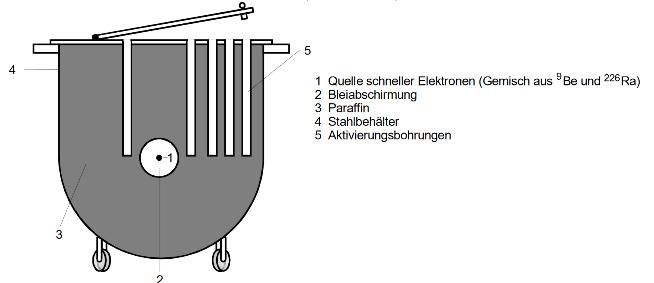
\includegraphics[scale=0.5]{content/images/neutronen.jpg}
\caption{Schematische Darstellung eines Behälters zu Anreicherung von radioaktiven Isotopen\cite{V702}}
\label{fig:ne}
\end{figure}

\subsection{Zerfallsreihen radioaktiver Isotope}
Die entstandenen radioaktiven Isotope zerfallen danach, wie in Zerfallsreihe \eqref{eq:Zerfall} beschrieben, in andere Kerne.
Für Vanadium gilt beispielsweise die Zerfallsreihe
\begin{equation}
\ce{^{51}_{23}V} + \ce{^{1}_{0}n} \rightarrow \ce{^{52}_{23}V} \rightarrow \ce{^{52}_{24}Cr} +  \beta^- + \bar{\nu}_.e
\end{equation}
Es gibt jedoch auch andere Kerne, bei denen mehrere Zerfallsprozesse möglich sind.
Hier soll beispielhaft Rhodium betrachtet werden.\newline
Durch den Beschuss mit Neutronen kann das stabile $\ce{^{103}_{45}Rh}$ zunächst zu einem angeregten Zwischenkern $\ce{^{104i}_{45}Rh\text{*}}$ wie in Reaktionsreihe \eqref{eq:Anregung} umgewandelt werden und erst anschließend weiter zerfallen. Die Wahrscheinlichkeit, dass dieser Fall eintritt liegt bei $10\%$.
Die andere Möglichkeit ist das der Zwischenkern keinen erhöhten Energiezustand hat, sondern direkt weiter zerfällt. Die Wahrscheinlichkeit dafür liegt bei $90\%$.
\begin{equation}
\ce{^{103}_{45}Rh} + \ce{^{1}_{0}n}
\begin{cases}
\underrightarrow{10\%}\ce{^{104i}_{45}Rh\text{*}}\rightarrow \ce{^{104}_{45}Rh}+ \gamma \rightarrow \ce{^{104}_{45}Pd} + \beta^- + \bar{\nu}_.e \\
\underrightarrow{90\%}\ce{^{104}_{45}Rh}\rightarrow \ce{^{104}_{45}Pd} + \beta^- + \bar{\nu}_.e
\end{cases}
\end{equation}
Da das angeregte $\ce{^{104i}_{45}Rh\text{*}}$ nur eine sehr kurze Halbwertszeit $\tau$ hat, wird zu Beginn der Messung die Aktivität sehr hoch. Es kann jedoch $\tau$ nicht exakt bestimmt werden, da parallel die andere Zerfallsreihe stattfindet und auch die bereits zerfallenen  $\ce{^{104i}_{45}Rh\text{*}}$ weiter zerfallen.
Es entsteht also eine Überlagerung der beiden Zerfälle.

\subsection{Messung der Halbwertszeit}

Wie bereits erwähnt ist es nicht möglich das Verhalten eines einzelnen Kerns vorherzusagen. Nur für große Mengen lässt sich eine statistische Aussage treffen.
Für die Anzahl $N$ der noch nicht zerfallen Kerne gilt:
\begin{equation}
N(t)=N_.0\mathrm{e}^{-\lambda t},\label{eq:N}
\end{equation}
mit der Anzahl der zu Beginn der Messung vorhandenen Kerne $N_.0$ und der elementspezifischen Zerfallskonstante $\lambda$.
Da $\tau$ die Zeit ist nach der noch genau die Hälfte der Kerne vorhanden sind, ergibt sich mit Gleichung \eqref{eq:N}:
\begin{equation}
\tau=\frac{\ln{(2)}}{\lambda}\label{eq:T}
\end{equation}
Da es schwierig ist die Anzahl der verbliebenen Kerne zu einem Zeitpunkt $t$ zu bestimmen, sehr wohl aber die Anzahl $N_.{\Delta t}$ der in einem Zeitintervall $\Delta t$ auftretenden Zerfälle, folgt mit Gleichung \eqref{eq:N}:
\begin{equation*}
N_.{\Delta t}(t)=N_.0\left(1-\mathrm{e}^{-\lambda\Delta t}\right)\mathrm{e}^{-\lambda t}
\end{equation*}
und damit 
\begin{equation}
\ln{\left(N_.{\Delta t}(t)\right)} = \ln{\left(N_.0\left(1-\mathrm{e^{-\lambda\Delta t}}\right)\right)}-\lambda t\text{.}\label{eq:ln}
\end{equation}
Der erste Term ist konstant und somit dies eine lineare Funktion aus der mittels lineare Ausgleichsrechnung $\lambda$ bestimmt werden kann.
